\section*{Fundamentos - P.A}

\begin{questions}
  \question Determine $x$ de modo que $(x ; 2x + 1 ; 5x + 7)$ seja uma P.A.

  \vspace{0.5cm}

  \question Obtenha 3 números em P.A, de modo que a soma entre esses seja igual a 3 e a soma de seus quadrados seja 11

  \vspace{0.5cm}

  \question Os números que exprimem o lado, a diagonal e a área de um quadrado estão, respectivamente, em P.A. Determine quanto mede o lado.

  \vspace{0.5cm}

  \question Demonstre que se $(a, b, c)$ é uma P.A, então $(a^{2}bc, ab^{2}c, abc^{2})$ também é.

  \vspace{0.5cm}

  \question Determine qual é o primeiro termo negativo da P.A $f = \{60, 53, 46, \dots\}$.

  \vspace{0.5cm}

  \question Sabe-se que $a_{10} = 7$ e que $a_{12} = -8$. Monte a P.A.

  \vspace{0.5cm}

  \question  De 100 a 1000, quanto são os múltiplos de 2 ou 3.

  \vspace{0.5cm}

  \question Obtenha a soma dos 200 primeiros termos da sequência dos números ímpares positivos. Cálcule também a soma dos $n$ primeiros termos iniciais dessa mesma sequência.

  \vspace{0.5cm}

  \question Um jardineiro tem que regar 60 roseiras plantadas ao longo de uma vereda retilínea e distando 1 m uma da outra. Ele enche seu regador numa fonte situada na mesma vereda, a 15 m da primeira roseira, e a cada viagem rega 3 roseiras. Começando e terminando na fonte, determine qual é o percurso total que ele terá que caminhar até regar todas as roseiras.

  \vspace{0.5cm}

  \question \textbf{(ITA-SP)} Considere a progressão aritmética ($a_{1}, a_{2}, a_{3}, \dots, a_{50}$) de razão $d$. Se $\displaystyle \sum_{n = 1}^{10} a_{n} = 10 + 25d$ e $\displaystyle \sum_{n = 1}^{50} = 4550$. Então $d - a_{1}$ é igual a:
  \vspace{0.4cm}

  \begin{oneparchoices}
    \choice 3
    \choice 6
    \choice 9
    \choice 11
    \choice 14
  \end{oneparchoices}

\end{questions}

\section*{Fundamentos - P.G}

\begin{questions}

  \question Prove que se $x, y, z$, nessa ordem, formam uma P.G, vale a relação

  \[(x + y + z)(x - y + z) = x^{2} + y^{2} + z^{2}\]

  \vspace{0.5cm}

  \question Os lados de um triângulo retângulo apresentam medidas em P.G. Determine o valor de $q$.

  \vspace{0.5cm}

  \question Dada uma P.G finita $(a_{1}, a_{2}, \dots, a_{10})$ onde $a_{1} = 2$ e $a_{2} = 6$, então determine se $(a_{10})^{\frac{1}{8}} = 3\cdot (2)^{\frac{1}{8}}$ é uma sentença verídica.

  \vspace{0.5cm}

  \question Prove que se $(a_{1}, a_{2}, a_{3}, \dots)$ é P.G, então $\displaystyle \left(\frac{1}{a_{1}}, \dots\right)$ também é.

  \vspace{0.5cm}

  \question Determine $\displaystyle \sum_{i = 3}^{n} 2^{i} = 4088$

  \vspace{0.5cm}

  \question Sabendo que $0 < q < 1$, calcule o valor da expressão da P.G infinita

  \[q + 2q^{2} + 3q^{3} + \dots\]

  \question \textbf{(IME–RJ)} Uma placa metálica com base $b$ e altura $h$ sofre sucessivas reduções da sua área, em função da realização de diversos cortes, conforme ilustrado na figura abaixo. A cada passo, a área à direita é removida e a placa sofre um novo corte. Determine a soma das áreas removidas da placa original após serem realizados $n$ cortes.

  \begin{center}
  \begin{figure}[ht]
    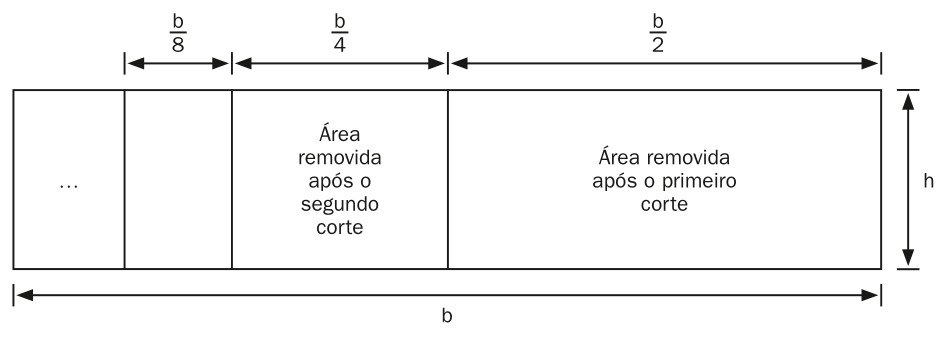
\includegraphics[width=12cm]{contents/ime-questao6}
    \centering
  \end{figure}
  \end{center}

  \question \textbf{(ITA-SP)} Seja $(a_{1}, a_{2}, \dots)$ uma progressão geométrica de razão $0 < a_{1} < 1$ e soma igual a $3a_{1}$. A soma dos três primeiros termos dessa progressão geométrica é igual a

  \vspace{0.3cm}

  \begin{oneparchoices}
    \choice $\displaystyle \frac{8}{27}$

    \choice $\displaystyle \frac{20}{27}$

    \choice $\displaystyle \frac{26}{27}$

    \choice $\displaystyle \frac{30}{27}$

    \choice $\displaystyle \frac{38}{27}$
  \end{oneparchoices}

  \vspace{0.5cm}

  \question \textbf{(Dep. de Matemática da Clínica Espiritual de Marabá - PA)} Para que os produtos dos termos da sequência

  \[\left(1, \sqrt{3}, \sqrt{3}^{2}, \sqrt{3}^{3}, \dots \sqrt{3}^{(n - 1)}\right)\]

  Seja igual a $3^{14}$, deverão ser consideradas, nessa sequência:

  \vspace{0.3cm}

  \begin{oneparchoices}
    \choice 8 termos
    \choice 6 termos
    \choice 10 termos
    \choice 9 termos
    \choice 7 termos
  \end{oneparchoices}

  \vspace{0.5cm}

  \question \textbf{(ITA-SP)} A progressão infinita $(a_{1}, \dots, a_{n}, \dots)$ tem razão $r < 0$. Sabe-se que a progressão infinita $(a_{1}, \dots, a_{(5n + 1)}, \dots)$ tem soma 8 e a progressão infinita $(a_{1}, \dots, a_{(5n)}, \dots)$ tem soma 2. Determine a soma da progressão $(a_{1}, \dots, a_{n}, \dots)$

\end{questions}
